\documentclass{article}
\usepackage[bottom=2cm, right=1.5cm, left=1.5cm, top=2cm]{geometry}
\usepackage{amsmath}
\usepackage{amssymb}
\usepackage{amsthm}
\usepackage{enumitem}
\usepackage{exercise} % Exercises Style
\usepackage{graphicx}
\usepackage{caption}
\usepackage{environ}



% Enable Code
\usepackage{minted}
\let \extra T

\newcommand{\vect}[1]{\boldsymbol{#1}}
\DeclareMathOperator{\Tr}{Tr}
\DeclareMathOperator{\Cov}{Cov}
\DeclareMathOperator{\Var}{Var}
\DeclareMathOperator{\E}{E}

\usepackage{fancyhdr}
\newenvironment{solution}
  {\renewcommand\qedsymbol{$\blacksquare$}\begin{proof}[Solution]$ $}
  {\end{proof}}

\title{Solutions to Assignment 9}
\author{Rongfei Jin}
\begin{document}

\pagestyle{fancy}
\fancyhf{}%
\fancyhead[L]{\textbf{ DS5220 \ Assignment 9}}
\fancyhead[R]{\textbf{Rongfei Jin}}
\fancyfoot[C]{\thepage}%
\maketitle

1,2,3,5,6,7,13

\section*{Exercise 1}
\subsection*{(a)}
\begin{figure}[h]
    \centering
    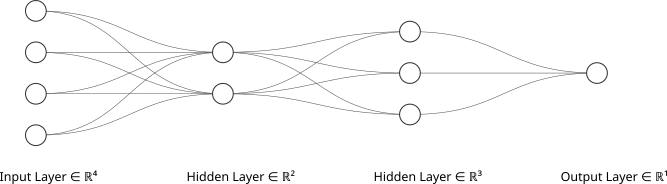
\includegraphics[width=0.5\textwidth]{figs/q1a.png}
    \caption{}
    \label{fig:}
\end{figure}

\subsection*{(b)}
First hidden layer
\[
A_k^{(1)} = (w_{k0}^{(1)} + \sum_{j=1}^{4} w_{kj}^{(1)}X_j)_+
\]

\begin{align*}
A_l^{(2)} &= (w_{l0}^{(2)} + \sum_{k=1}^{2} w_{lk}^{(2)} A_k^{(1)})_+ \\
A_l^{(2)} &= 
(w_{l0}^{(2)} + \sum_{k=1}^{2} w_{lk}^{(2)} 
(w_{k0}^{(1)} + \sum_{j=1}^{4} w_{kj}^{(1)}X_j)_+
)_+ \\
\end{align*}

\begin{align*}
Z &= (\beta_0 + \sum_{l=1}^{3} \beta_l A_l^{(2)})_+ \\
&= (\beta_0 + \sum_{l=1}^{3} \beta_l
(w_{l0}^{(2)} + \sum_{k=1}^{2} w_{lk}^{(2)} 
(w_{k0}^{(1)} + \sum_{j=1}^{4} w_{kj}^{(1)}X_j)_+
)_+)_+ \\
\end{align*}


\begin{align*}
f(X) 
&= \beta_0 + (\sum_{l=1}^{3}\beta_l A_l^{(2)})_+ \\
&= \beta_0 + (\sum_{l=1}^{3}\beta_l \sum_{j=1}^{2})(\beta_j)+ \\
\end{align*}

\subsection*{(c)}
\inputminted{r}{src/q1.R}

\subsection*{(d)}
The total number of parameters in the network is the sum of the parameters in each layer.
\[(4+1)\cdot 2 + (2+1)\cdot 3 + (1+3) = 23\]

\section*{Exercise 2}
\subsection*{(a)}

\begin{align*}
\frac{e^{Z_m+c}}{\sum_{l=0}^{L}e^{Z_l+c}} 
&= \frac{e^c}{e^c} \cdot \frac{e^{Z_m}}{\sum_{l=0}^{L} e^{Z_l}} \\
&= \frac{e^{Z_m}}{\sum_{l=0}^{L} e^{Z_l}} \\
\end{align*}

\subsection*{(b)}
\begin{align*}
\frac{e^{c_1 + \cdots + c_p + \beta_{k0} +\beta_{k_1x_1} + \cdots + \beta_{k_p x_p}}}{\sum_{l=1}^K e^{c_1 + \cdots + c_p + \beta_{l0} +\beta_{l_1x_1} + \cdots + \beta_{k_p x_p}}} 
&= \frac{e^{c_1 + \cdots + c_p} \cdot e^{\beta_{k0} +\beta_{k_1x_1} + \cdots + \beta_{k_p x_p}}}{e^{c_1 + \cdots + c_p}\cdot \sum_{l=1}^K  e^{\beta_{l0} +\beta_{l_1x_1} + \cdots + \beta_{l_p x_p}}} \\
&= \frac{e^{\beta_{k0} +\beta_{k_1x_1} + \cdots + \beta_{k_p x_p}}}{\sum_{l=1}^K e^{\beta_{l0} +\beta_{l_1x_1} + \cdots + \beta_{k_p x_p}}} \\
\end{align*}

\section*{Exercise 3}

\begin{align*}
-\sum_{i=1}^{n}\sum_{i=1}^{2}\log(f_m(x_i))
\end{align*}

\begin{align*}
\ell(\beta_0, \beta_1) &= \prod_{i:y_1 = 1}p(x_i) \prod_{i:y_1 = 0}(1-p(x_i)) \\
\log (\ell(\beta_0, \beta_1)) &= \sum_{i:y_1 = 1}\log(p(x_i)) + \sum_{i:y_1 = 0}\log(1-p(x_i)) \\
\end{align*}

Let \(f_1 = p(x), f_2 = (1-p(x))\), \(y_{i1}, y_{i0}\) be the indicator function for \(y_i = 1\) and \(y_i = 0\) respectively. Then we can rewrite the log-likelihood as:

\begin{align*}
\log (\ell(\beta_0, \beta_1)) &= \sum^{i}y_{i1} \log(p(x_i)) + \sum^i y_{i0} \log(1-p(x_i)) \\
\end{align*}

This is equivalent to the negative multinomial log-likelihood function 

\section*{Exercise 5}
\[
R^2 = 1 - \frac{\text{SSE}}{\text{SST}} = 1 - \frac{\sum_{i=1}^n (y_i - \hat{y}_i)^2}{\sum_{i=1}^n (y_i - \bar{y})^2}\]

\[
\text{MAE} = \frac{1}{n}\sum_{i=1}^n |y_i - \hat{y}_i|
\]

MAE does not square the error, so it is less sensitive to outliers than MSE. In contrast, \(R^2\) is a relative measure of fit that compares the variance explained by the model to the total variance in the data.


\newpage
\section*{Exercise 6}

\subsection*{(a)}
\begin{figure}[h]
    \centering
    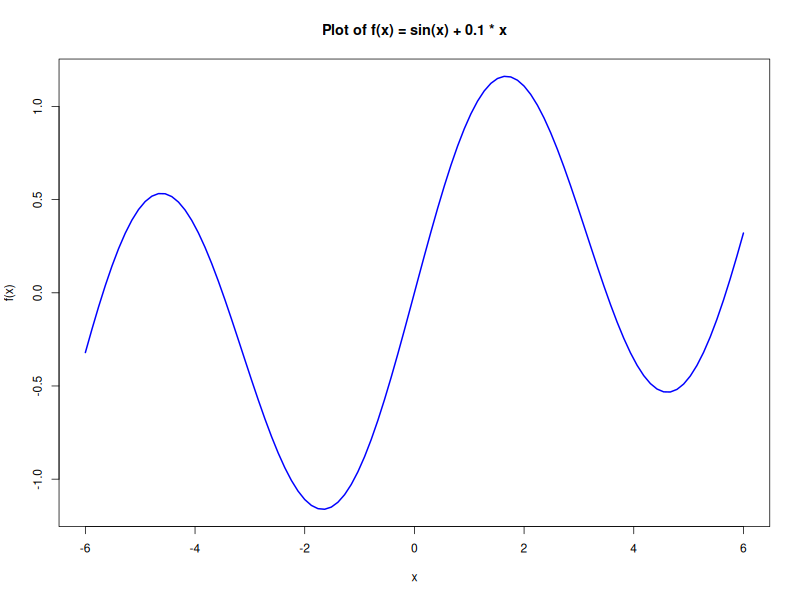
\includegraphics[width=0.5\textwidth]{figs/q6a.png}
    \caption{}
    \label{fig:q6a}
\end{figure}
\subsection*{(b)}
\[cos(\beta) + \frac{1}{10}\]
\subsection*{(c) and (d)}

\begin{figure}[h]
    \centering
    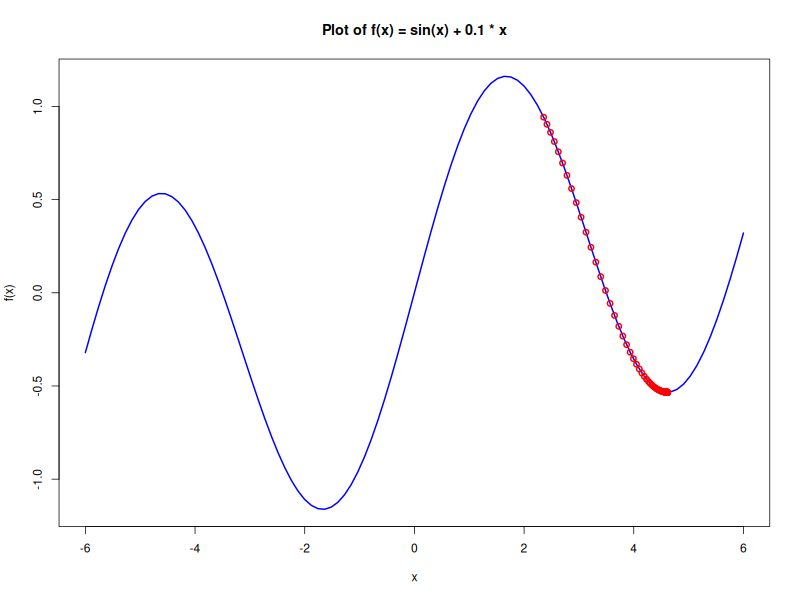
\includegraphics[width=0.5\textwidth]{figs/q6c.png}
    \caption{}
    \label{fig:q6c}
\end{figure}
\newpage

\begin{figure}[h]
    \centering
    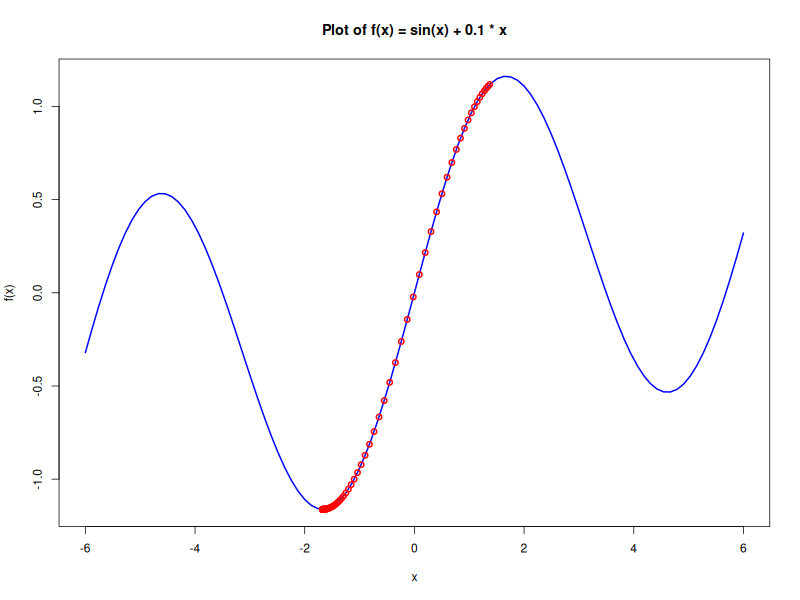
\includegraphics[width=0.5\textwidth]{figs/q6d.png}
    \caption{}
    \label{fig:q6d}
\end{figure}
\inputminted{r}{src/q6.R}

\newpage
\section*{Exercise 7}



\end{document}